\section{光滑化}
\label{sec:opt-ns-smoothing}

邻近方法要求非光滑项有便宜的邻近映射。有限个仿射函数的最大值$\max_i\{\bm a_i^\top\bm x+b_i\}$就常常没有：它的邻近子问题是一个二次规划。另一条路是放弃精确保留尖点，用一个光滑函数整体替换原目标，再调用第~\ref{chap:opt-smooth}章的光滑方法。这样做引入了两种误差：替代函数与原函数之间的偏差，以及替代问题没有求准的误差。本节先构造最大值的光滑替代并计算偏差，再说明怎样在两种误差之间分配精度。

\subsection{最大值的光滑逼近}
\label{sec:opt-ns-smooth-max}

最大值函数的尖点出现在活跃分支切换的地方：在切换点一侧，梯度是一个分支的斜率；越过切换点，梯度立刻跳到另一个分支的斜率。要得到光滑函数，就要让这种切换在一个小范围内连续地完成。

\paragraph{对数和指数光滑化}
设$\varphi(\bm x)=\max_{1\leq i\leq m}\ell_i(\bm x)$，其中$\ell_i(\bm x)=\bm a_i^\top\bm x+b_i$。给定平滑参数$\nu>0$，令
\begin{equation}
 \varphi_\nu(\bm x)=\nu\log\sum_{i=1}^m\exp\Bigl(\frac{\ell_i(\bm x)}\nu\Bigr).
 \label{eq:opt-ns-lse}
\end{equation}
它称为对数和指数（log-sum-exp）\term{光滑化}（smoothing）。直观上，指数把较大的分支放大得远比较小的分支多，$\nu$越小，求和越由最大的那一项主导，对数再把它还原回原来的尺度。

偏差可以精确控制。记$M=\varphi(\bm x)$，把$e^{M/\nu}$提到求和号外：
\[
 \varphi_\nu(\bm x)=M+\nu\log\sum_{i=1}^m\exp\Bigl(\frac{\ell_i(\bm x)-M}\nu\Bigr).
\]
求和中每一项都在$(0,1]$内，并且取到最大值的那一项等于$1$，所以和介于$1$与$m$之间。于是对所有$\bm x$，
\begin{equation}
 \varphi(\bm x)\leq\varphi_\nu(\bm x)\leq\varphi(\bm x)+\nu\log m .
 \label{eq:opt-ns-lse-gap}
\end{equation}
偏差不依赖$\bm x$，也不依赖$\bm a_i,b_i$，只依赖分支数和$\nu$。

\paragraph{梯度与曲率}
对式~\eqref{eq:opt-ns-lse}求导，得
\[
 \nabla\varphi_\nu(\bm x)=\sum_{i=1}^mp_i(\bm x)\,\bm a_i,\qquad
 p_i(\bm x)=\frac{\exp(\ell_i(\bm x)/\nu)}{\sum_{k=1}^m\exp(\ell_k(\bm x)/\nu)} .
\]
权重$p_i$非负、和为$1$，是各分支的软化选择：活跃分支的权重最大，离活跃越远的分支权重以指数速度衰减。再求一次导数，Hessian为
\[
 \nabla^2\varphi_\nu(\bm x)=\frac1\nu\Bigl(\sum_ip_i\bm a_i\bm a_i^\top-\bar{\bm a}\bar{\bm a}^\top\Bigr),\qquad\bar{\bm a}=\sum_ip_i\bm a_i ,
\]
括号中是以$p_i$为权重的斜率协方差矩阵。它半正定，并且在半正定序下不超过$\sum_ip_i\bm a_i\bm a_i^\top$，后者又不超过$\max_i\lVert\bm a_i\rVert_2^2\,\bm I$。所以$\varphi_\nu$是凸函数，并且是$L_\nu$光滑的，$L_\nu=\max_i\lVert\bm a_i\rVert_2^2/\nu$。偏差界与光滑常数一起显示了平滑参数的两面：$\nu$越小，偏差$\nu\log m$越小，曲率上界$1/\nu$却越大，梯度方法可用的步长随之缩小。

\begin{example}[绝对值的两种光滑化]
\label{ex:opt-ns-abs-smoothing}
$|x|=\max\{x,-x\}$有$m=2$个分支。对数和指数光滑化为
\[
 \varphi_\nu(x)=\nu\log\bigl(e^{x/\nu}+e^{-x/\nu}\bigr),\qquad\varphi_\nu'(x)=\tanh(x/\nu),
\]
偏差在$x=0$处最大，等于$\nu\log2$。另一种常用的替代是Huber函数
\[
 h_\nu(x)=\begin{cases}x^2/(2\nu),&|x|\leq\nu,\\|x|-\nu/2,&|x|>\nu,\end{cases}\qquad h_\nu'(x)=\min\{\max\{x/\nu,-1\},1\},
\]
它把尖点附近长度为$2\nu$的一段换成抛物线，从下方逼近$|x|$，偏差$|x|-h_\nu(x)$在$[0,\nu/2]$内。两种替代的二阶导数都不超过$1/\nu$。图~\ref{fig:opt-ns-smooth-max}画出$\nu=0.5$时的情形。
\end{example}

\begin{figure}[!htbp]
  \centering
  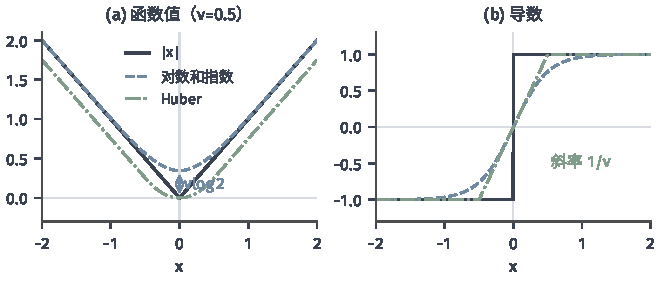
\includegraphics[width=112mm]{figures/03-optimization-evolution-and-signals/01-optimization/matplotlib/c4-smooth-max/figure.pdf}
  \caption{绝对值的两种光滑化（$\nu=0.5$）。(a) 黑线是$|x|$，蓝色虚线是对数和指数光滑化，从上方逼近，在原点的偏差为$\nu\log2\approx0.35$；绿色点划线是Huber函数，从下方逼近，偏差不超过$\nu/2$。(b) 对应的导数：$|x|$的导数在原点跳变，$\tanh(x/\nu)$与截断的直线$x/\nu$都连续地完成从$-1$到$1$的过渡，过渡区的斜率不超过$1/\nu$。}
  \label{fig:opt-ns-smooth-max}
\end{figure}

Huber函数最早作为稳健估计中的损失提出\sidecite{huber1964}，这里只用它的光滑性。图~\ref{fig:opt-ns-smooth-max}右图值得细看：原函数的导数在原点处从$-1$跳到$1$，两种替代都在宽度约为$\nu$的区间内连续地走完这段跳变。$\nu$减半，过渡区间变窄一半，过渡段的斜率加倍，这正是$L_\nu\propto1/\nu$的来源。

\paragraph{Huber函数是Moreau包络}
Huber函数并不是凭空设计的。对适当、下半连续的凸函数$f$，令
\[
 e_\nu f(\bm x)=\min_{\bm y}\Bigl\{f(\bm y)+\frac1{2\nu}\lVert\bm y-\bm x\rVert_2^2\Bigr\},
\]
称为$f$的\term{Moreau包络}（Moreau envelope）。它就是第~\ref{sec:opt-ns-prox}节邻近子问题的最优值，最小点是$\operatorname{prox}_{\nu f}(\bm x)$。对$f=|\cdot|$，代入软阈值：$|x|\leq\nu$时最小点是$0$，最优值为$x^2/(2\nu)$；$|x|>\nu$时最小点是$p=x-\nu\operatorname{sign}(x)$，$|p|=|x|-\nu$，距离项为$\nu^2/(2\nu)=\nu/2$，最优值为$|x|-\nu/2$。这正是$h_\nu$。一般地，Moreau包络是可微凸函数，梯度为$\bigl(\bm x-\operatorname{prox}_{\nu f}(\bm x)\bigr)/\nu$，且梯度是$1/\nu$-Lipschitz的\sidecite[第31节]{rockafellar1970convex}；对$|x|$可以直接验证：$\bigl(x-\operatorname{sign}(x)\max\{|x|-\nu,0\}\bigr)/\nu=h_\nu'(x)$。所以只要邻近映射可算，就能得到一个光滑替代；而对没有便宜邻近映射的最大值函数，对数和指数光滑化给出了另一条显式途径。

\paragraph{替代梯度不是原次梯度}
光滑化后，算法读取的是$\nabla\varphi_\nu(\bm x)=\sum_ip_i\bm a_i$。在远离切换点的地方，它接近活跃分支的斜率；在切换点附近，它是所有分支的软加权平均，这个向量一般不属于原函数在该点的次微分。例如$|x|$在$x=0.1$处的次微分是$\{1\}$，而$\nu=0.5$时$\tanh(0.2)\approx0.197$。因此光滑化方法不是“次梯度法换了一种选次梯度的方式”：它在每一轮求解的都是当前的光滑函数$\varphi_\nu$，收敛的对象也是$\varphi_\nu$的最小点，而不是原函数的最小点。两者之间的差距，要靠偏差界~\eqref{eq:opt-ns-lse-gap}来控制。

\subsection{偏差与求解精度}
\label{sec:opt-ns-smoothing-budget}

设原目标为$F=\phi+\varphi$，其中$\phi$是凸且$L_\phi$光滑的函数（可以为零），$\varphi$是上面的有限仿射最大值。用$F_\nu=\phi+\varphi_\nu$代替$F$，它是凸的且$(L_\phi+\max_i\lVert\bm a_i\rVert_2^2/\nu)$光滑。设$\widehat{\bm x}$是对$F_\nu$求解后返回的点，$F^\star$与$F_\nu^\star$分别是两个函数的最小值。

\paragraph{误差分解}
由式~\eqref{eq:opt-ns-lse-gap}，$F(\widehat{\bm x})\leq F_\nu(\widehat{\bm x})$；又对原问题任一最小点$\bm x^\star$，$F_\nu^\star\leq F_\nu(\bm x^\star)\leq F^\star+\nu\log m$。两式相减，
\begin{equation}
 F(\widehat{\bm x})-F^\star\leq\bigl(F_\nu(\widehat{\bm x})-F_\nu^\star\bigr)+\nu\log m .
 \label{eq:opt-ns-smoothing-split}
\end{equation}
右端第一项是替代问题的优化误差，可以靠增加迭代次数减小；第二项是替代本身的偏差，只取决于$\nu$。对固定的$\nu$，即使把替代问题完全求解，第二项仍然留在那里。

\paragraph{分配精度}
给定原目标的精度要求$\varepsilon$，自然的分配是两项各占一半：取$\nu=\varepsilon/(2\log m)$使偏差不超过$\varepsilon/2$，再把替代问题求解到优化误差不超过$\varepsilon/2$。设$\phi=0$、替代问题的最小点到初值的距离不超过$R$。第~\ref{chap:opt-smooth}章对凸$L$光滑目标给出：步长$1/L$的梯度下降$T$步后目标差不超过$LR^2/(2T)$，加速梯度法不超过$2LR^2/(T+1)^2$。代入$L_\nu=\max_i\lVert\bm a_i\rVert_2^2/\nu=2\log m\,\max_i\lVert\bm a_i\rVert_2^2/\varepsilon$，梯度下降需要约$L_\nu R^2/\varepsilon=O(\varepsilon^{-2})$次梯度计算，加速方法需要约$R\sqrt{4L_\nu/\varepsilon}=O(\varepsilon^{-1})$次。后者优于次梯度法的$O(\varepsilon^{-2})$次查询，但它依赖显式的最大值结构：每次梯度计算都要算出全部$m$个分支，任意的黑箱非光滑函数没有这种结构。

\begin{example}[固定平滑参数的平台]
\label{ex:opt-ns-smoothing-plateau}
在平面上取$m=5$个分支，斜率是单位圆上等分的五个方向$\bm a_i=(\cos\frac{2\pi(i-1)}5,\sin\frac{2\pi(i-1)}5)^\top$，截距$\bm b=(0,0.3,-0.2,0.5,0.1)^\top$。用线性规划求得原问题的最小值$F^\star\approx0.3065$。对$\nu=1,\ 0.1,\ 0.01$分别从$(3,2)^\top$出发，以步长$\nu$（即$1/L_\nu$）对$F_\nu$做梯度下降，并记录原目标的误差$F(\bm x^{(t)})-F^\star$。图~\ref{fig:opt-ns-smoothing-budget}显示：$\nu=1$时误差在10步内就降到约$0.09$并停住；$\nu=0.1$时约40步后停在约$0.026$；$\nu=0.01$时要约400步才开始快速下降，最终停在约$0.0026$。三个平台都在各自的偏差界$\nu\log5$（点线）以下。$\nu$越小，平台越低，但步长同样按$\nu$缩小，到达平台所需的步数也越多。
\end{example}

\begin{figure}[!htbp]
  \centering
  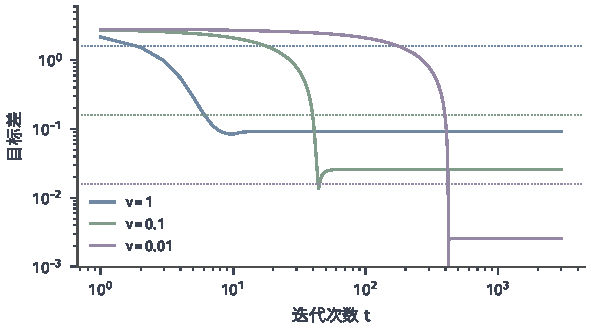
\includegraphics[width=100mm]{figures/03-optimization-evolution-and-signals/01-optimization/matplotlib/c4-smoothing-budget/figure.pdf}
  \caption{固定平滑参数的梯度下降在原目标上的误差（例~\ref{ex:opt-ns-smoothing-plateau}，双对数坐标）。蓝、绿、紫三条曲线分别对应$\nu=1,0.1,0.01$，步长均为$\nu$；同色点线是偏差界$\nu\log5$。每条曲线最终停在由$\nu$决定的平台上；$\nu$越小，平台越低，到达平台所需的迭代越多。}
  \label{fig:opt-ns-smoothing-budget}
\end{figure}

\paragraph{改变平滑参数}
实践中常从较大的$\nu$开始，得到粗略解后再缩小$\nu$，用上一阶段的结果作初值。每次缩小$\nu$，光滑常数$L_\nu$随之增大，必须重新确定步长，不能沿用旧$\nu$下的步长；相应的停止精度也要按新的偏差重新分配，新增的梯度计算要计入总预算。

\paragraph{替代目标下降，原目标未必下降}
梯度方法保证的是$F_\nu$的下降，原目标$F$可以在某一轮上升。再看例~\ref{ex:opt-ns-three-pieces}的$f(x)=\max\{-x,x/2,2x-3\}$，取$\nu=1$，$L_\nu\leq\max_ia_i^2/\nu=4$，步长$1/4$。从原问题的最小点$x=0$出发：三个分支在$0$处的值是$0,0,-3$，权重正比于$1,1,e^{-3}$，替代梯度为
\[
 \varphi_\nu'(0)=\frac{-1+\frac12+2e^{-3}}{2+e^{-3}}\approx-0.195 ,
\]
一步后到达$x\approx0.049$。替代函数值从$\log(2+e^{-3})\approx0.718$降到约$0.709$，原目标却从最小值$0$升到约$0.024$。原因是$F_\nu$的最小点不在$0$：$x/2$分支的软权重把它向右拉开了一段。式~\eqref{eq:opt-ns-lse-gap}只保证上升不超过$\nu\log m$，不保证逐轮不升。因此光滑化方法应同时记录替代目标和原目标，按式~\eqref{eq:opt-ns-smoothing-split}判断最终输出，而不是要求每一轮原目标都改善；这与下一节的代理模型不同，那里每轮都要用原目标检验改善。
